\documentclass[conf]{new-aiaa}
%\documentclass[journal]{new-aiaa} for journal papers
\usepackage[utf8]{inputenc}

\usepackage{graphicx}
\usepackage{amsmath}
\usepackage[version=4]{mhchem}
\usepackage{siunitx}
\usepackage{longtable,tabularx}
\usepackage{float}
\usepackage{csvsimple}
\setlength\LTleft{0pt} 

\title{Project 2}
\author{Mauro Patimo}
\begin{document}
\maketitle

\section{Nomenclature}

{\renewcommand\arraystretch{1.0}
\noindent\begin{longtable*}{@{}l @{\quad=\quad} l@{}}
$f$  & equation introduced in similarity solution \\
$f'$ & derivative of f with respect to $\eta$ \\
$\eta$ & variable introduced in similarity solution to relate y and x\\
$\Lambda$ & constant introduced in similarity solution \\
$\beta$ & parameter introduced in Falkner-Skan equation \\
$\delta^*$ & displacement thickness \\
$\theta$ & momentum thickness \\
$C_f$ & skin friction coefficient \\
$H$ & shape factor \\
$Re_{\theta}$ & Reynolds number based on momentum thickness \\
$g(x)$ & shape factor for Pohlhausen approximation \\
$U_e$ & free stream velocity \\

\end{longtable*}}

\section{Introduction}
Different methods can be used to calculate the velocity profile of a boundary layer.
Falkner-Skan equations are a set of nonlinear differential equations that describe the flow of a viscous, incompressible fluid over a flat plate. The equations are a generalization of the Blasius equation, which is obtained by setting the pressure gradient to zero. \\
The following paper will present a numerical solution to the Falkner-Skan equations for different values of the parameter $\beta$. 
The results will be compared to the Pohlhausen approximation and the Thwaites-Walz method.\\
The Pohlhausen approximation is a method used to calculate the velocity profile of a boundary layer. It is a simplification of the Falkner-Skan equations, which are a set of nonlinear differential equations that describe the flow of a viscous, incompressible fluid over a plate. The equations are a generalization of the Blasius equation, which is obtained by setting the pressure gradient to zero. \\
\section{Procedure}
The Falkner-Skan equation is:
\begin{equation}
    f'''+ff''+\beta(1-f'^2)=0
\end{equation}
With the following boundary conditions:
\begin{equation}
    f(0)=f'(0)=0, \quad f'(\infty)=1
\end{equation}
$f(0)$ and $f'(0)$ are set equal to zero due to the no-slip boundary condition. $f'(\infty)$ is set equal to 1 due to the free stream condition, where the flow's velocity parallel to the surface approaches $U_e$ when it is infinitely far away from the surface, in our case $\eta=100$. \\
The equations are solved numerically using the shooting method. The initial conditions are guessed and the equations are solved. If the value of $f''(\infty)\neq 0$ the initial conditions are then adjusted by using the secant method to find the roots of our equation, until the boundary conditions are satisfied. \\
\section{Results}
\begin{figure}[H]
    \centering
    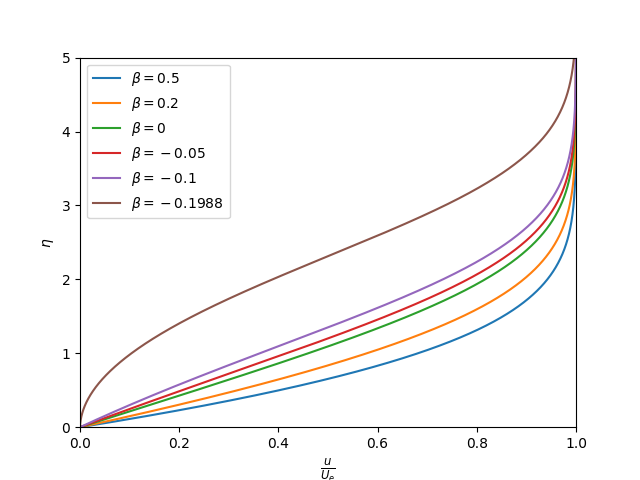
\includegraphics[width=0.5\textwidth]{Project 2.png}
    \caption{Falkner-Skan flow for different betas}
    \label{fig:Falkner-Skan for different betas}
\end{figure}

\begin{figure}[H]
    \centering
    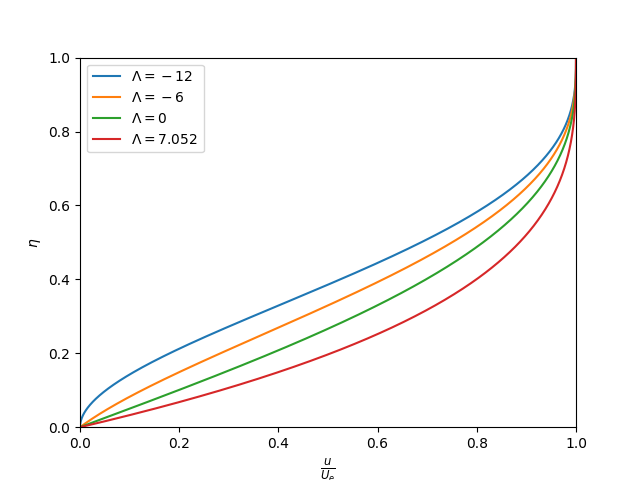
\includegraphics[width=0.5\textwidth]{Pohlhausen.png}
    \caption{Pohlhausen approximation}
    \label{fig:Falkner-Skan}
\end{figure}

\begin{center}
    \resizebox{0.40\linewidth}{!}{\begin{tabular}{rrrr}
\hline
   $\beta$ &   $\frac{\theta}{g(x)}$ &   $c_f Re_{\theta}$ &     $H$ \\
\hline
    0.5    &                0.350299 &          0.649846   & 2.2958  \\
    0.2    &                0.408342 &          0.560824   & 2.40849 \\
    0      &                0.469342 &          0.440563   & 2.59369 \\
   -0.05   &                0.490107 &          0.392059   & 2.67814 \\
   -0.1    &                0.514655 &          0.328216   & 2.80418 \\
   -0.1988 &                0.575706 &          0.00547205 & 3.98866 \\
\hline
\end{tabular}}\label{tab:table1}
\end{center}

\begin{figure}[H]
    \centering
    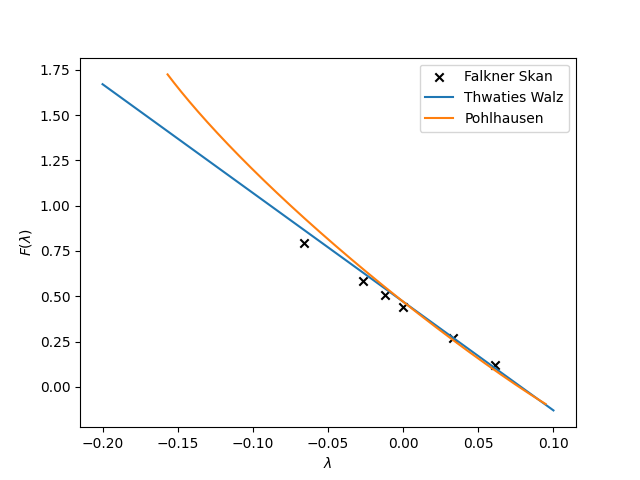
\includegraphics[width=0.5\textwidth]{Thwaites Walz.png}
    \caption{Different profile methods}
    \label{fig:multiple profiles}
\end{figure}
\section{Discussion and Conclusion} \label{sec:conclusion}
The displacement thickness is calculated using the following equation:
\begin{equation}
   \frac{\delta^\star}{g(x)}=\lim_{\eta \to \infty} \eta -f
\end{equation}
The momentum thickness is calculated using the following equation:
\begin{equation}
    \frac{\theta}{g(x)} = \frac{f''(0)}{1+\beta}-\frac{\beta}{1+\beta}\frac{\delta^*}{g(x)}
\end{equation}
This value increases with $\beta$ because the velocity profile tends to increase in thickness. If we imagine a 2D flow, in order to have lower $\beta$ we need to have an decrease in the slope of the surface, meaning that the area the flow can occupy increases  and therefore it can slow down in order due to the conservation of mass. 
A lower need for the velocity to increase quickly means a smaller momentum \\
The skin fiction coefficient is calculated using the following equation:
\begin{equation}
    C_f=\frac{2}{Re_{\theta}}\frac{d^2f}{d\eta^2}\Big|_{\eta=0}\frac{\theta}{g(x)}
\end{equation}
A higher skin friction coefficient means a higher drag coefficient. This is due to the fact that the skin friction coefficient is proportional to the shear stress, which is proportional to the drag force. It is quantifiable in the plot by looking at the slope of the velocity profile in relation to the height, the more horizontal the velocity profile the higher the skin-friction coefficient.\\
The shape factor is calculated using the following equation:
\begin{equation}
    H=\left(\frac{\theta}{g(x)}\right)^{-1} \left(\lim_{\eta \to \infty} \eta-f\right)
\end{equation}
It describes the shape of the velocity profile. A lower H value is present when $\beta$ values are higher because the flow is more turbulent and the boundary layer is thinner. \\
As expected all the profiles plotted in Fig. \ref{fig:multiple profiles} are very similar. The Thwaites-Walz profile is a good approximation that simplifies our calculations and improves the running time of the scripts, in addition to being very easy to mentally visualize. 
However, the calculations for out Falkner-Skan profile take less than 1.5 seconds for 6 different values of beta, so the time constraint is not an issue. \\
Furthermore, the values shown in Table \ref{tab:table1} are within a reasonable error of the actual values. This also affects very slightly the plot in Fig. \ref{fig:multiple profiles}. \\
The Pohlhausen approximation is a good approximation for the Falkner-Skan profile, but it is not as accurate as the Thwaites-Walz profile. \\
\appendix
\section{Appendix}
As mentioned in \ref{sec:conclusion} since the time constraint is not an issue we can calculate the Falkner-Skan profile for many different type of $\beta$. Fig. \ref{fig:Falkner-Skan multiples betas} is an example of 40 values of $\beta$ in between $-0.1988$ and $0.5$. The runtime of the script to obtain this plot is about 5 seconds.
\begin{figure}[H]
    \centering
    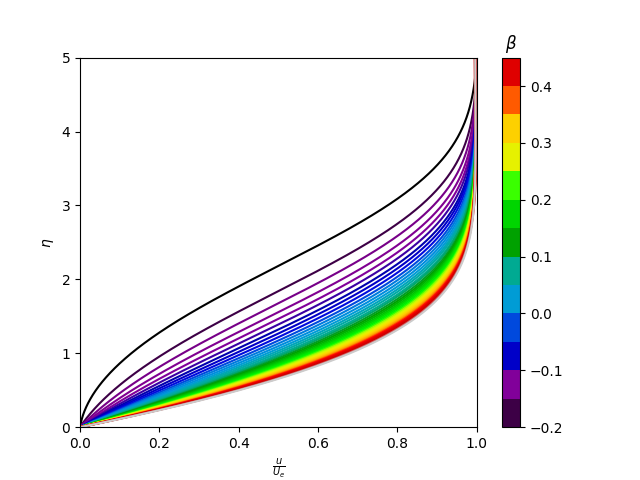
\includegraphics[width=0.5\textwidth]{Continuous beta.png}
    \caption{Falkner-Skan flow for different betas}
    \label{fig:Falkner-Skan multiples betas}
\end{figure}
\end{document}
